\chapter{Testing}\label{ch:testing}

The testing phase of this parking management system follows a comprehensive approach as outlined in \cref{ch:methodology_approach}, beginning with individual component testing before progressing to integrated system validation. This methodical approach ensures that each component functions correctly in isolation before examining their interaction within the complete system.

\section{Individual Tests}

The database testing phase focused on ensuring data integrity and proper relationship management through rigorous SQL query testing. Multiple database iterations were conducted to refine data categories and verify correct data representation. Critical tests included validating constraints such as boolean attributes being limited to 0 and 1 values, and ensuring logical consistency in numerical fields like preventing negative values for parking space allocations. This thorough validation process helped establish a robust foundation for data storage and manipulation.

The terminal testing concentrated on validating the API endpoints using Insomnia \autocite{insomnia2025}, a specialized tool for API testing and documentation. Each endpoint underwent systematic testing to verify correct functionality, proper error handling, and expected response formats. This process generated comprehensive documentation of API behaviors and interactions, creating a valuable reference for future development and maintenance. See \cref{fig:insomnia} for reference.

\begin{figure}
        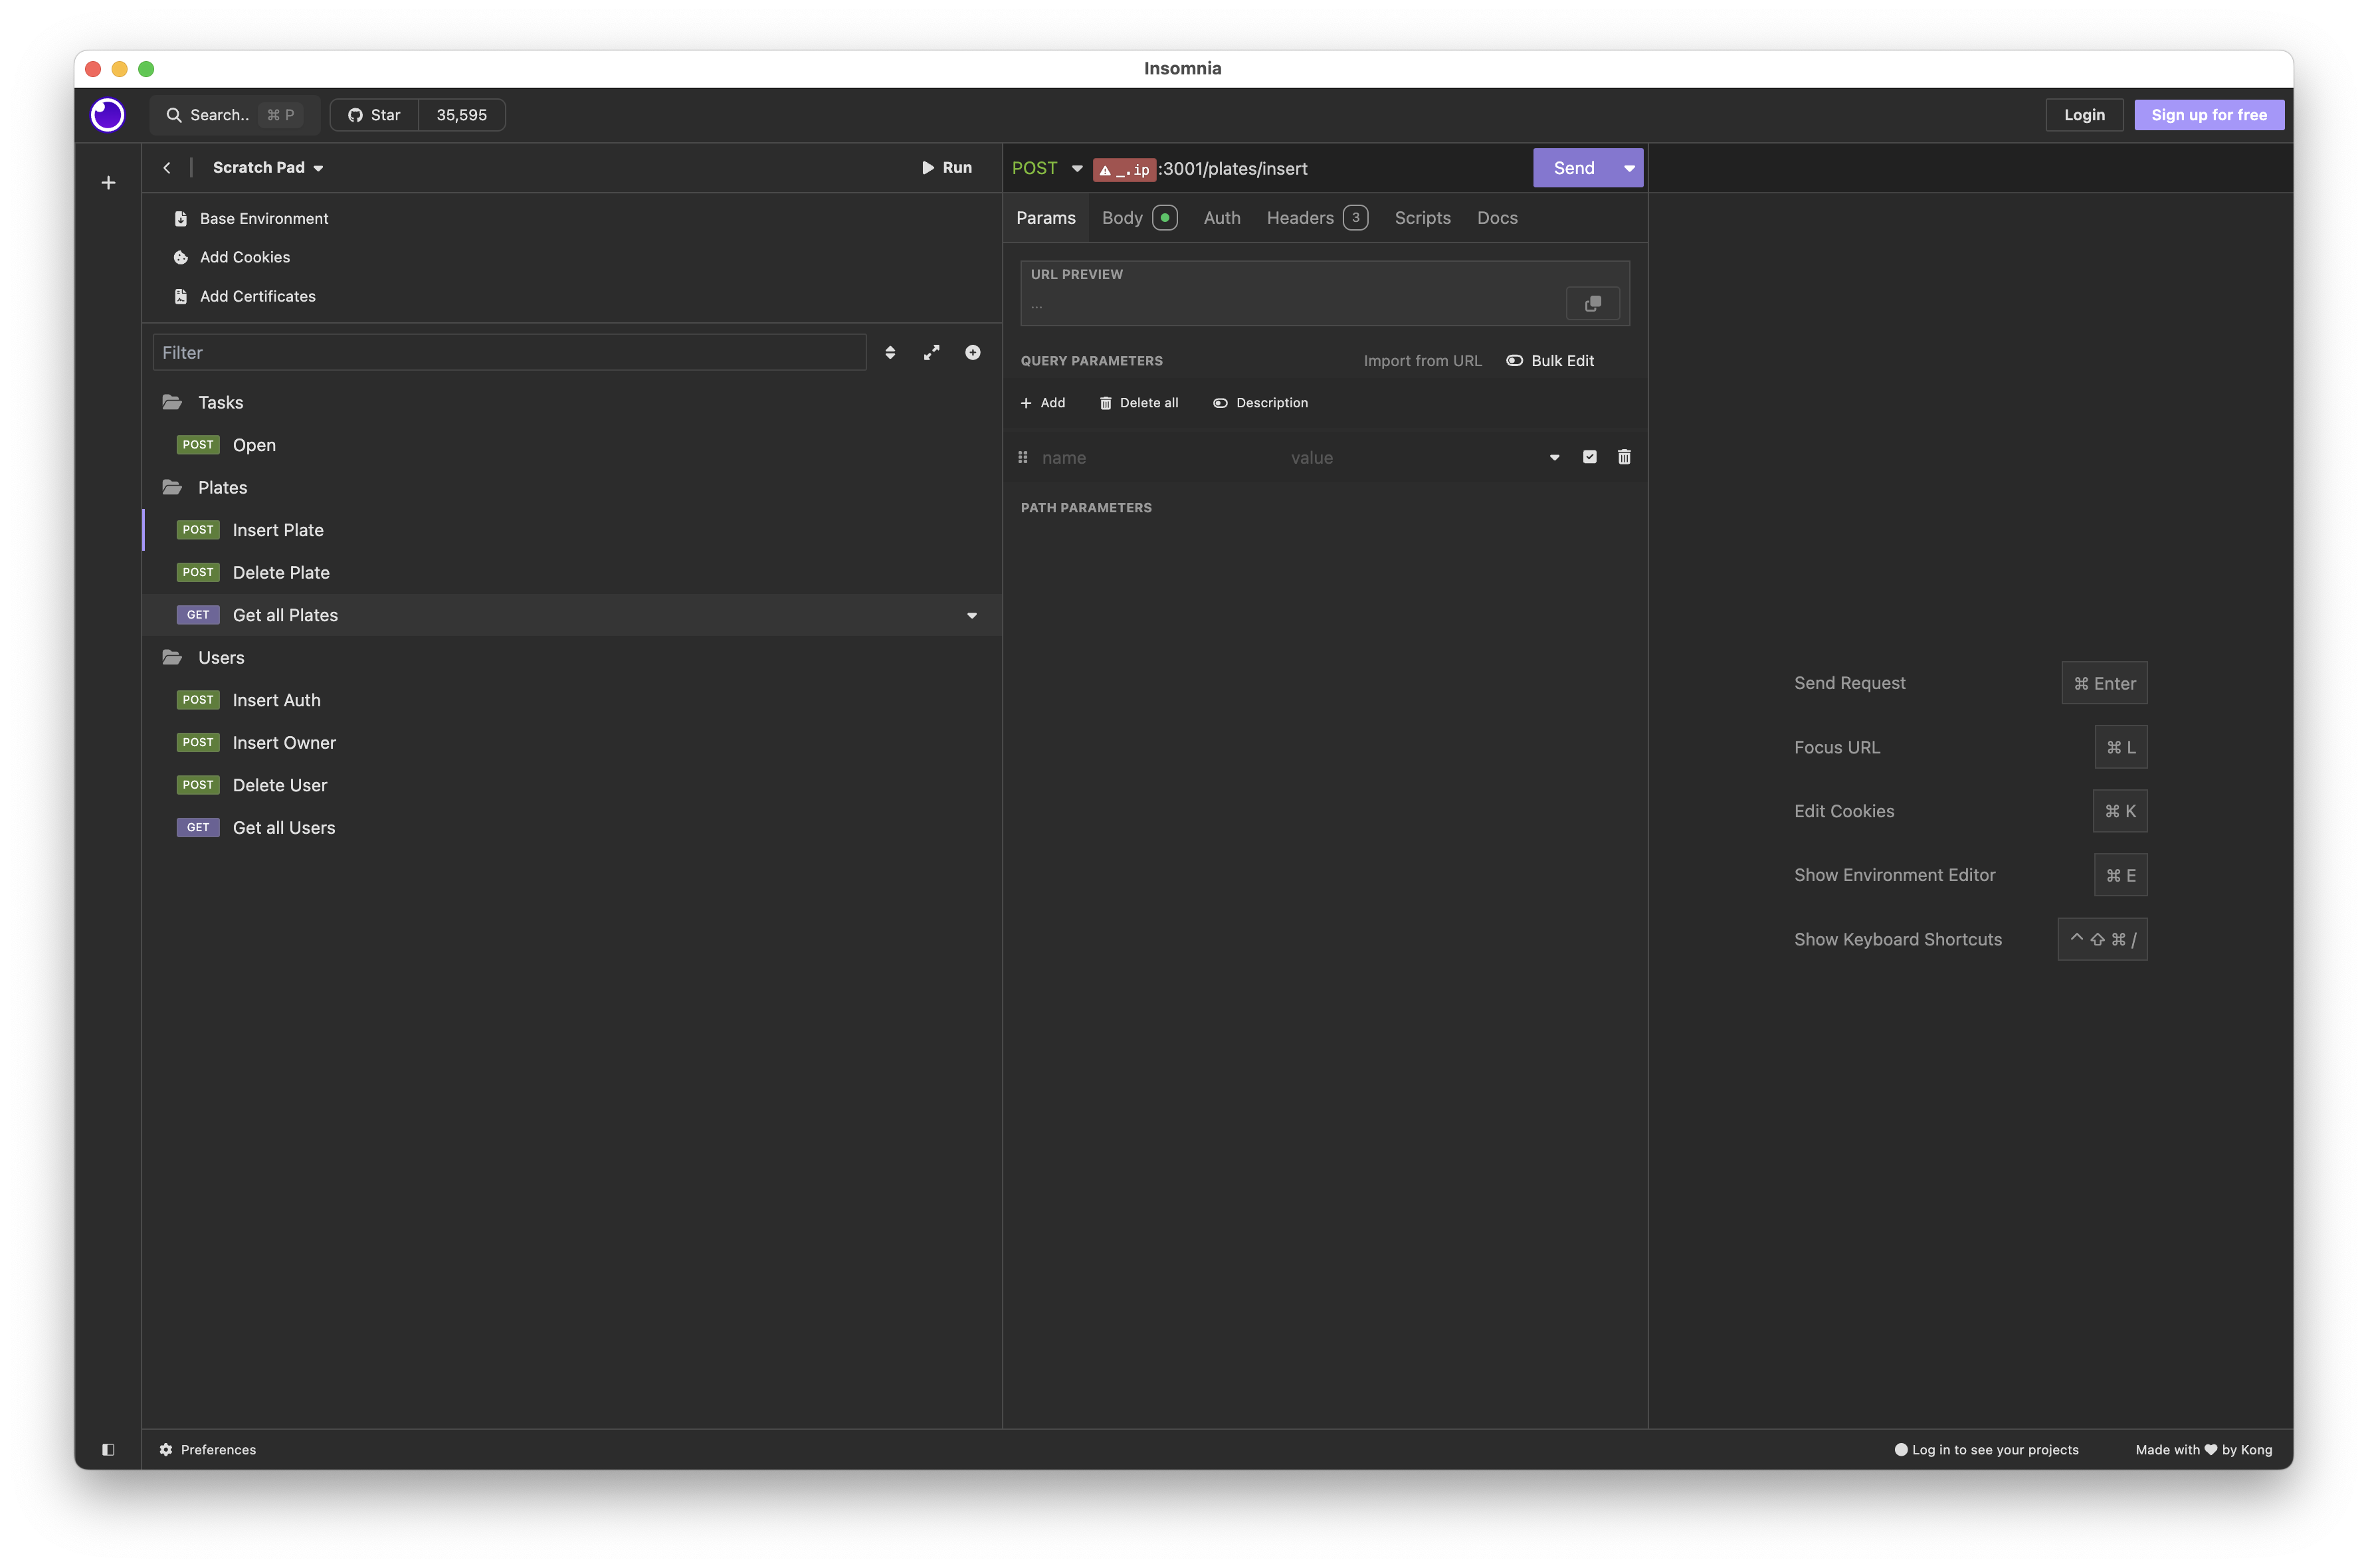
\includegraphics{insomnia.png}
    \caption{Testing API endpoints using Insomnia}\label{fig:insomnia}
\end{figure}

Server testing incorporated both visual interface validation and functional integration testing. The visual testing focused on ensuring proper website rendering across different devices and screen sizes using the Responsive Design Mode available in Firefox and Google Chrome's developer tools. Additionally, extensive integration testing was performed to verify seamless communication between the server and terminal components in a local environment.j

Moreover, the ML model testing phase involved evaluating the model's accuracy and performance under various conditions. This included testing the model's ability to predict parking space availability based on historical data and real-time inputs. The model was subjected to stress tests to assess its robustness and scalability, ensuring reliable performance in a production environment. This is out of the scope of this document, but more information can be found in the project's GitHub repository \autocite{RAMAJOBALLESTER2024104608}.

\section{Controlled Environment Tests}

Once the different components were tested individually, the system was deployed in a controlled environment to evaluate its performance under realistic conditions. This phase involved simulating parking lot scenarios to assess the system's ability to manage parking space availability, process user requests, and provide accurate information in real-time. The controlled environment tests helped identify potential bottlenecks, refine system behavior, and optimize performance.

For this, the system was built inside a register and installed in a facility in Valencia, Spain, see \cref{fig:installation_testing}. This installation box allowed for controlled testing of the system's hardware components, including the infrared sensors, cameras, and LED displays. The system's performance was evaluated under different lighting conditions, weather scenarios, and parking lot configurations to ensure reliable operation in diverse environments.

\begin{figure}
	\hfill
	\begin{subfigure}{0.45\textwidth}
		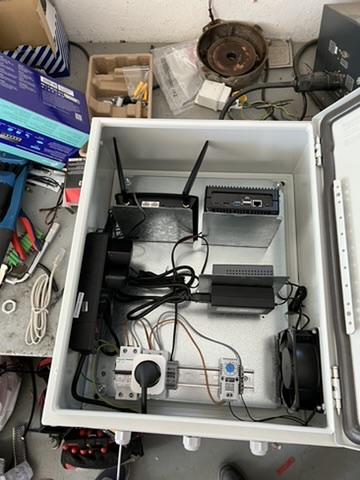
\includegraphics{installation_box.jpg}
		\caption{Installation box for the parking management system}
	\end{subfigure}
	\hfill
	\begin{subfigure}{0.45\textwidth}
		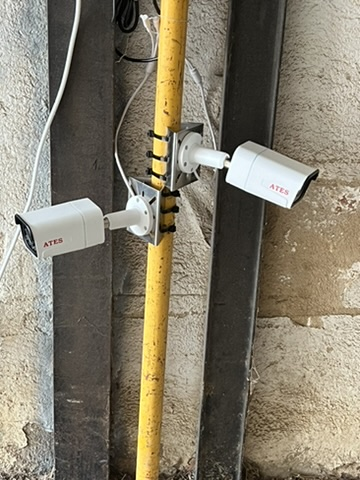
\includegraphics{installation_cameras.jpg}\label{fig:installation_cameras}
		\caption{Installation of cameras for the parking management system}.
	\end{subfigure}
	\hfill

	\caption{Installation testing.}\label{fig:installation_testing}
\end{figure}

The testing phase highlighted several areas requiring additional attention, particularly regarding network reliability and hardware interactions. These findings led to important system refinements and the development of robust fallback mechanisms to maintain system functionality under suboptimal conditions. The problems encountered during the testing phase are detailed in the following subsections.

\subsection{Network Connectivity Issues}

Real-world deployment highlighted challenges related to network connectivity. The selection of appropriate cellular network providers was crucial for ensuring system reliability in diverse environments. Movistar generally provided better coverage in underground parking areas, while Orange offered more robust connectivity in urban settings. Frequent switching between providers was necessary to ensure continuous operation. 

Network resilience was tested by simulating poor connection quality and complete connection loss. The system demonstrated its ability to maintain local functionality during network outages, caching data and synchronizing with the central server once connectivity was restored. However, these tests revealed the need for improved error handling and user feedback mechanisms to clearly indicate network status. 

The reliance on 4G connectivity introduced dependencies on external infrastructure, which was a major limitation. To mitigate this issue, redundant communication paths, such as local Wi-Fi networks, were explored as backup options. Automated switching between cellular and Wi-Fi networks would enhance system resilience and ensure continuous operation even when one network becomes unavailable.

\subsection{Hardware Interactions}

Hardware testing revealed initial inconsistencies in the relay system used for garage door control. The relays, responsible for actuating the door mechanisms, exhibited unreliable behavior, especially in environments with fluctuating humidity levels. The original setup proved sensitive to moisture, leading to intermittent failures and potentially disrupting the seamless operation of the parking system. 

To address this, a custom Relay Expansion Board was used and integrated with the NVIDIA Jetson Nano, see \cref{fig:relay_expansion_board}. This expansion board not only provided more robust relays better suited to handle varying environmental conditions but also facilitated a more streamlined and reliable connection between the control system and the physical door mechanisms. The new relays were chosen for their higher tolerance to humidity and their ability to maintain consistent performance over extended periods. This upgrade ensured smoother and more dependable garage door operations.

\begin{figure}
	\hfill
	\begin{subfigure}{0.45\textwidth}
		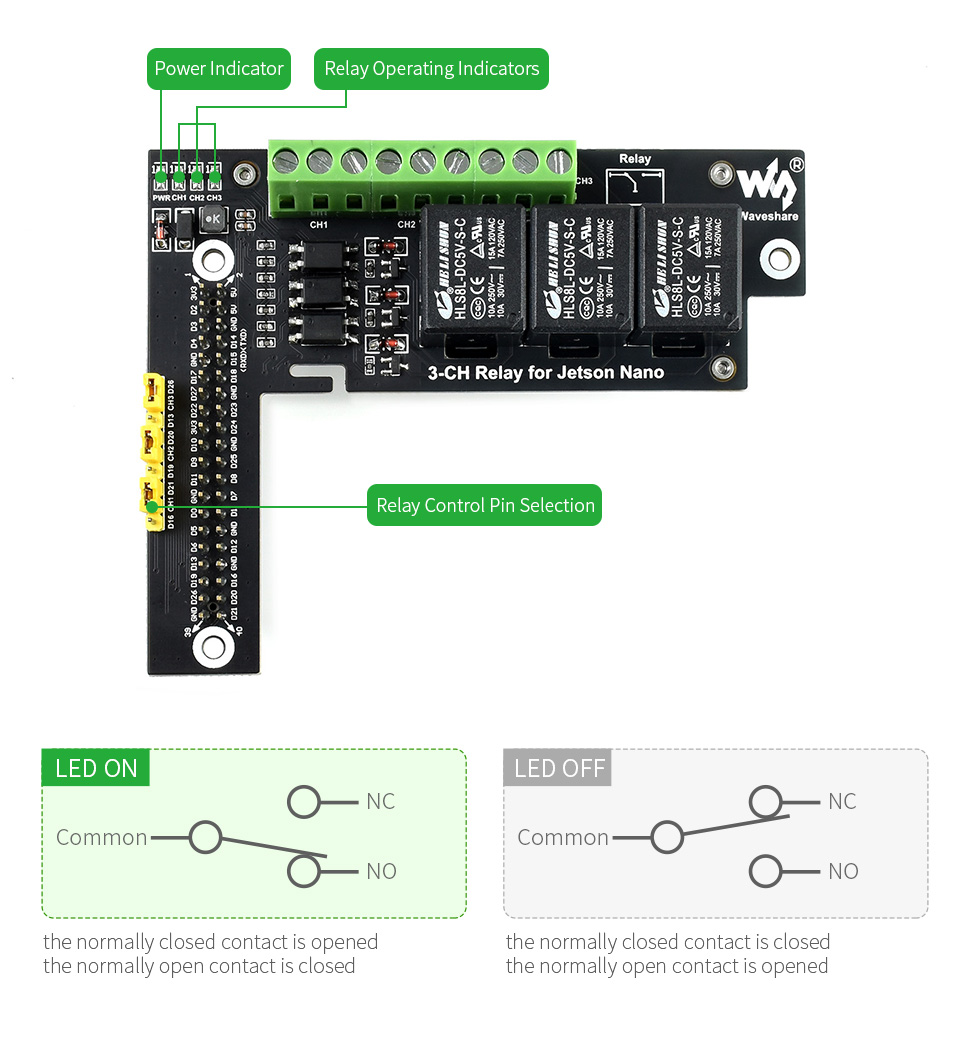
\includegraphics{rele_doc.jpg}
	\end{subfigure}
	\hfill
	\begin{subfigure}{0.45\textwidth}
		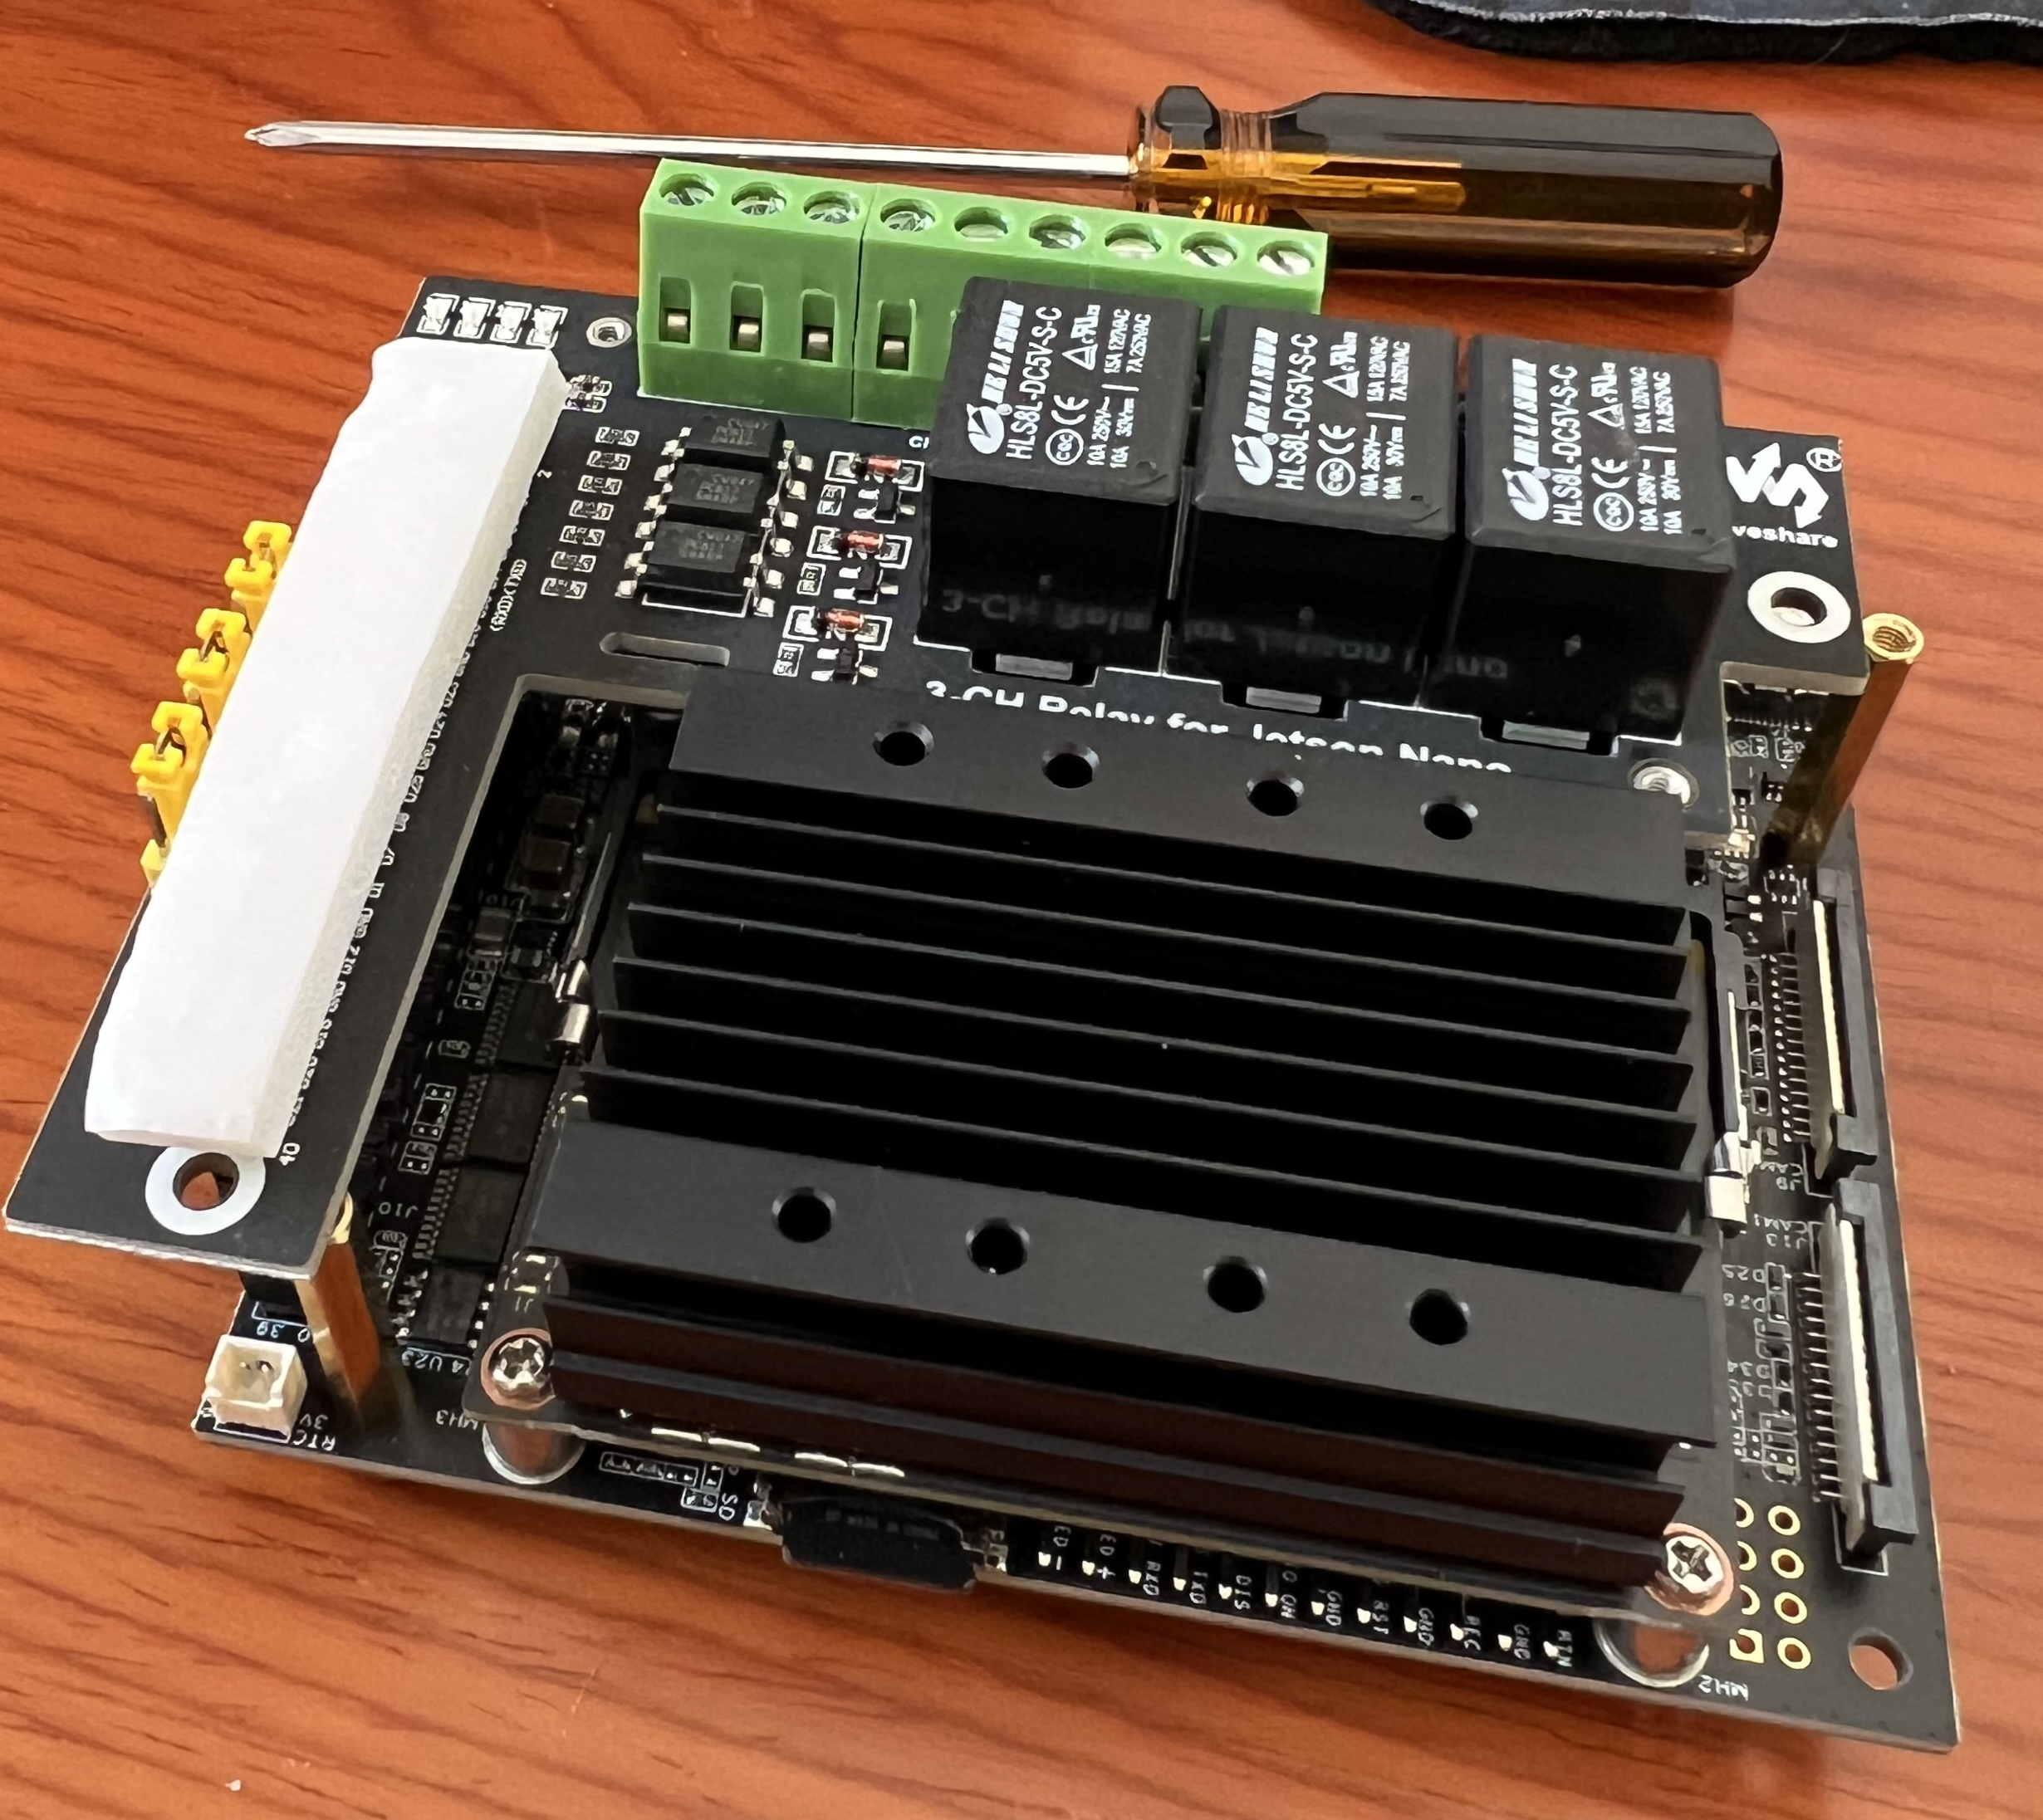
\includegraphics{reles.jpg}
	\end{subfigure}
	\hfill

	\caption{Relay Expansion Board for garage door control.}\label{fig:relay_expansion_board}
\end{figure}


\subsection{Low Light Conditions}

The system's ability to accurately detect license plates was tested under various lighting conditions, including low light environments. The initial tests showed that the system struggled to reliably identify license plates when the lighting was poor. This was mainly due to the limitations of the cameras' infrared capabilities as it only provided a visible flash of light, which was insufficient for capturing clear images in dark areas, see \cref{fig:night_without_infrared}.

To address this, additional infrared lighting was strategically placed to supplement the cameras' built-in infrared capabilities, which significantly improved license plate recognition in poorly lit areas, see \cref{fig:night_with_infrared}. Different camera models were also tested. Further optimization of the image processing algorithms was done to enhance contrast and clarity in low light images. For reference, the infrared light used is a 8-Light Illuminator Infrared08E of 8 W of power and a wavelenght of 850 nm.

\begin{figure}
	\begin{subfigure}{0.95\textwidth}
		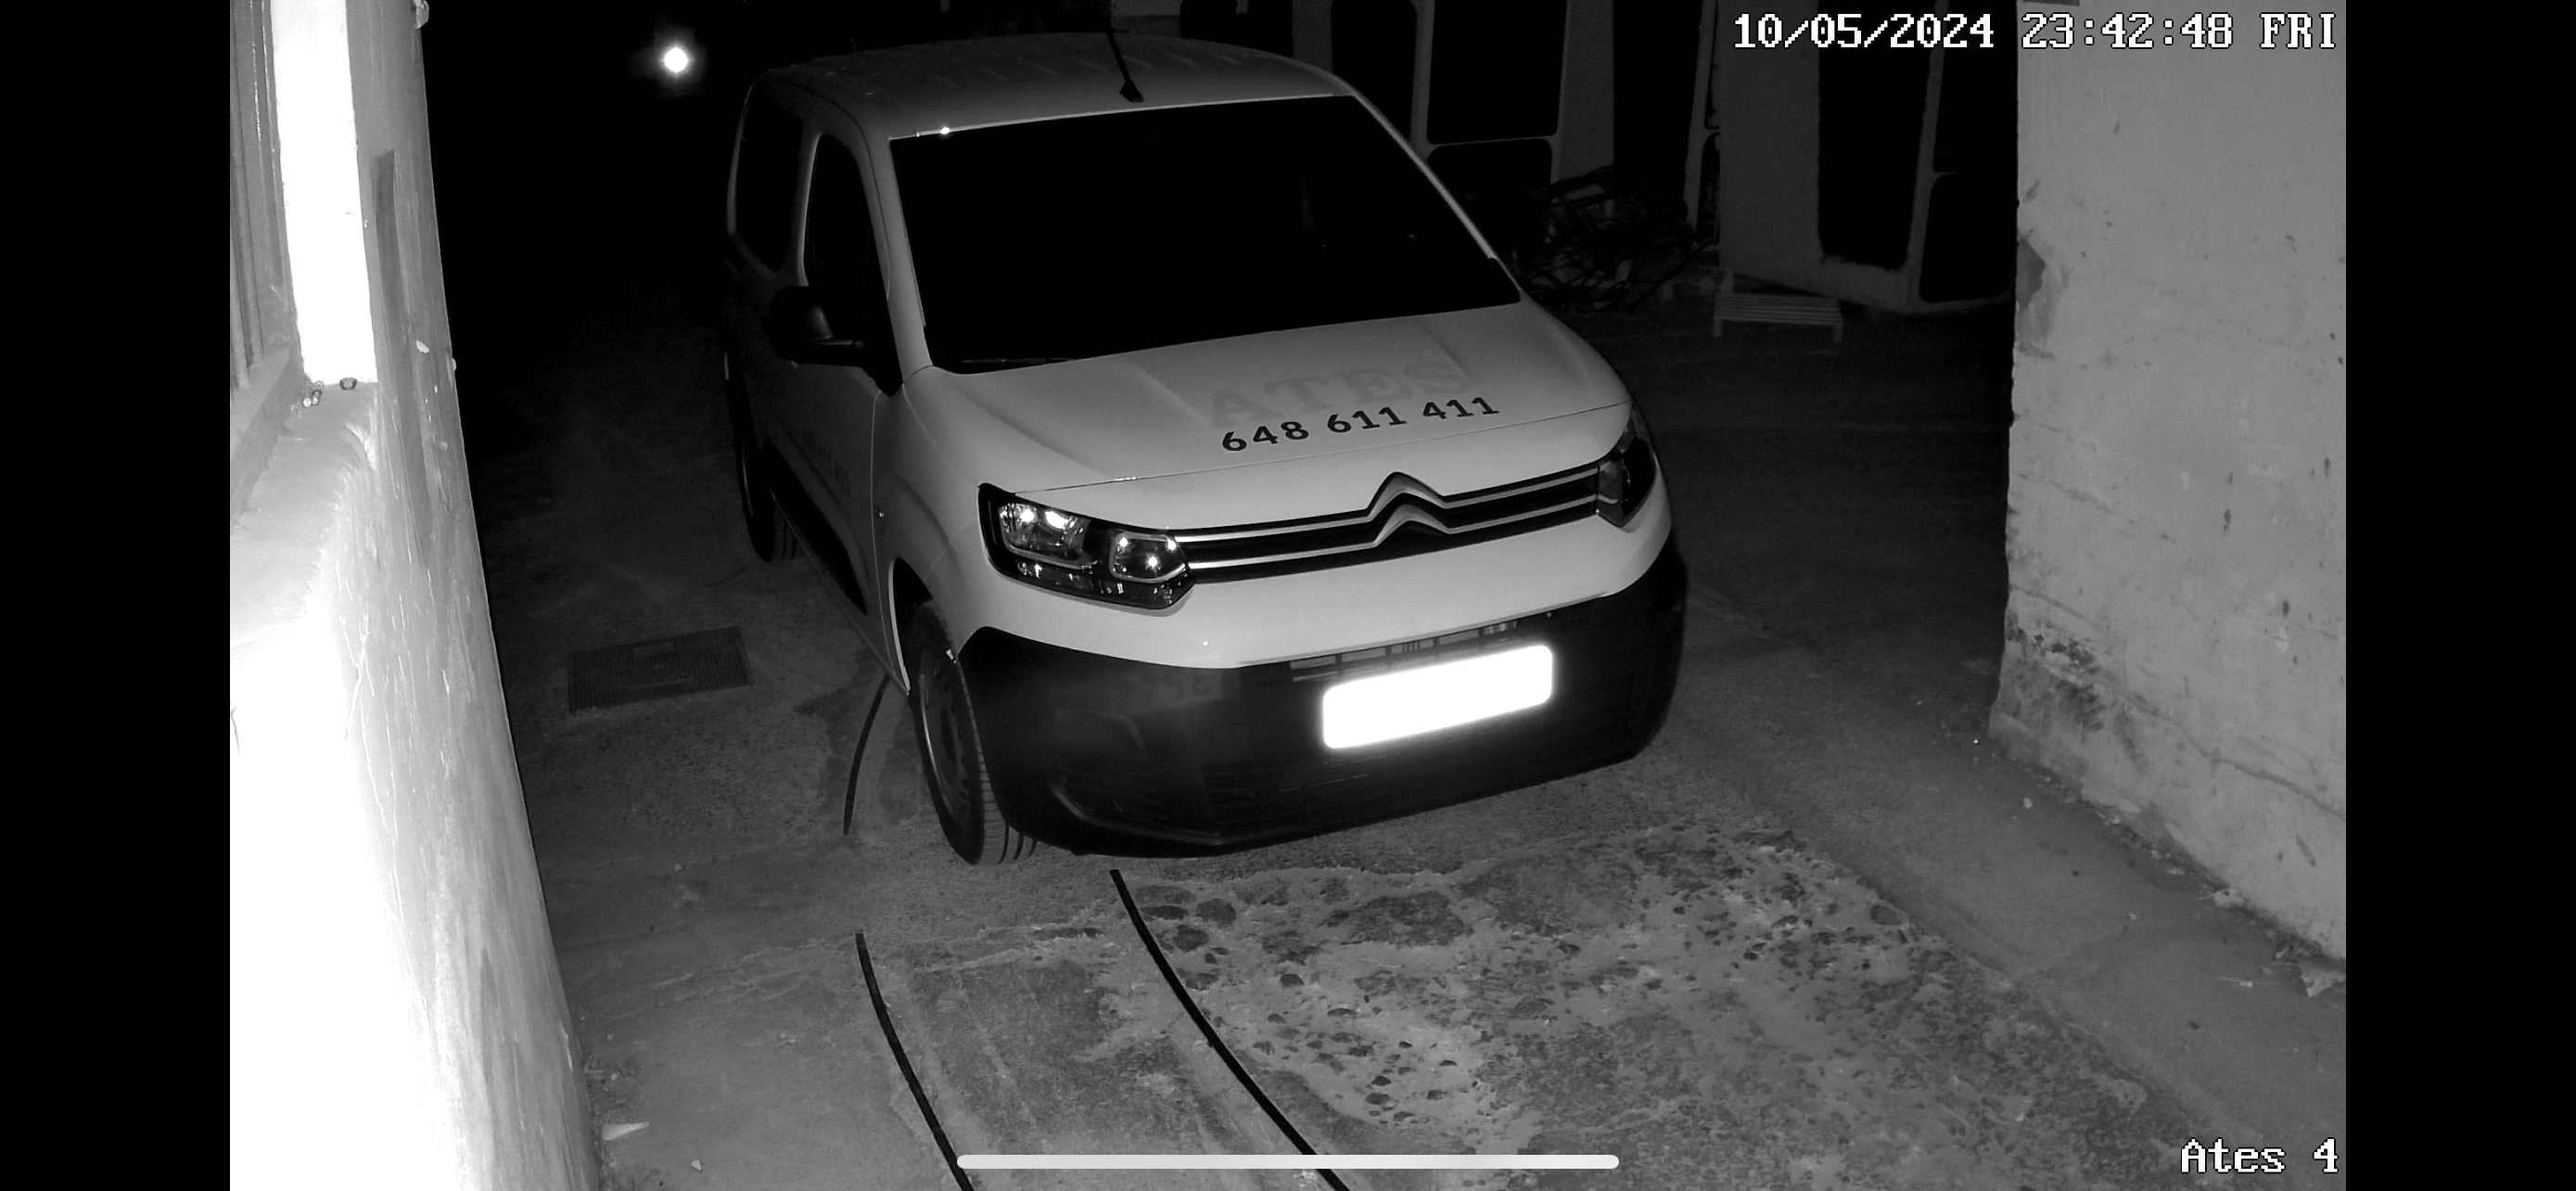
\includegraphics{night_without_infrared.png}
		\caption{Image captured at night without infrared lighting.}\label{fig:night_without_infrared}
	\end{subfigure}
    \br
	\begin{subfigure}{0.95\textwidth}
		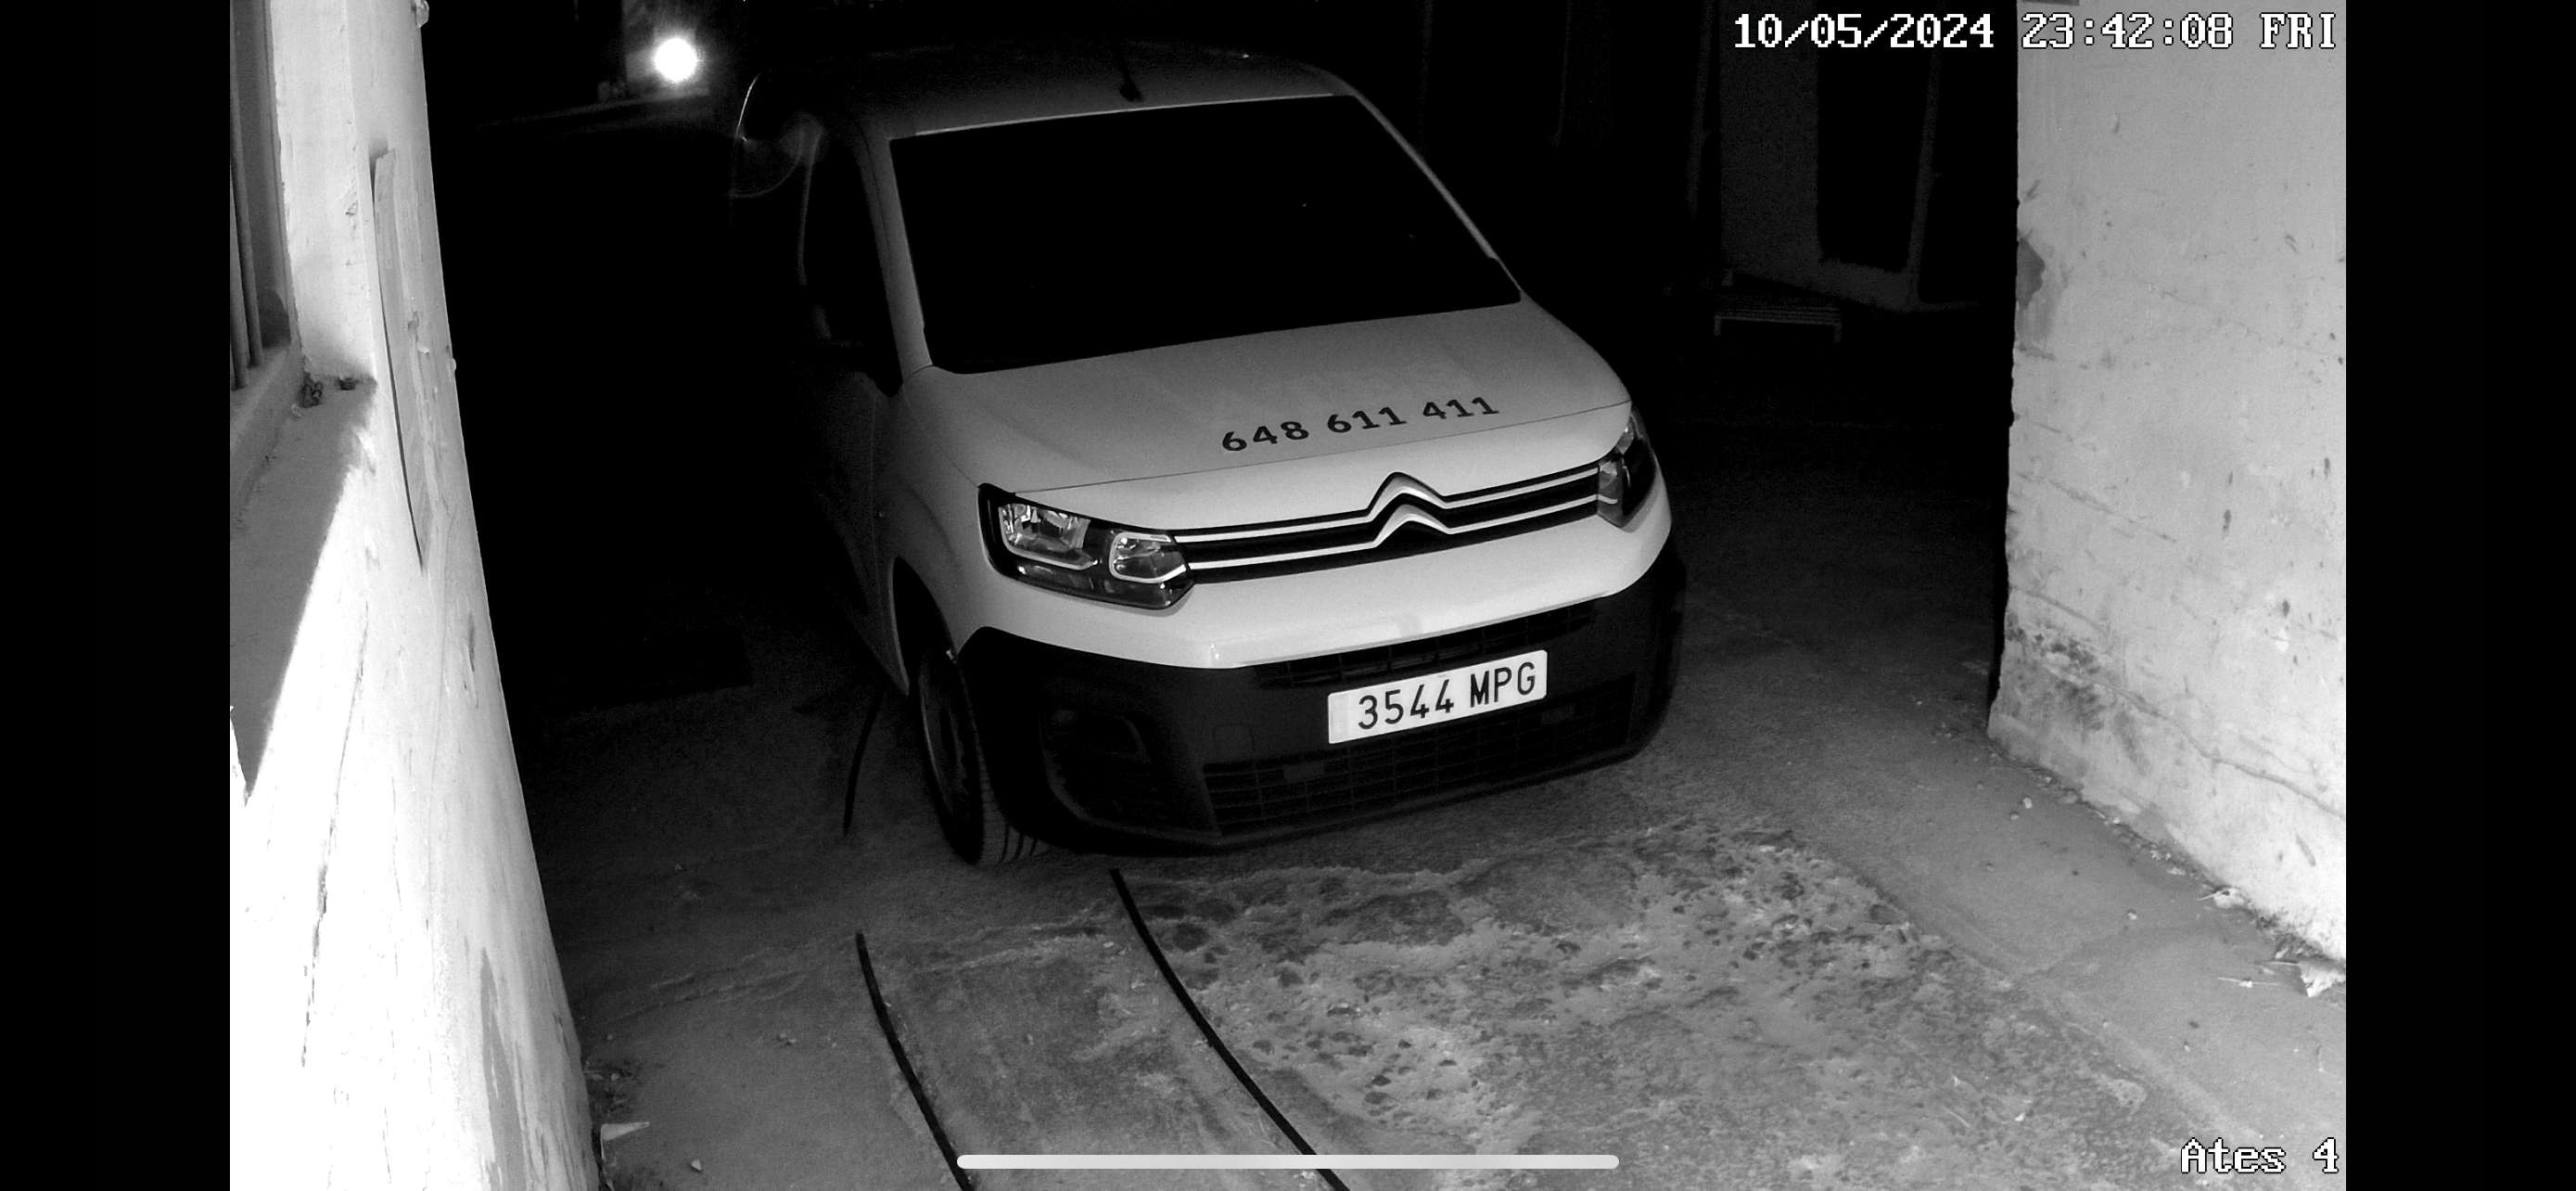
\includegraphics{night_with_infrared.png}
		\caption{Image captured at night with infrared lighting installed.}\label{fig:night_with_infrared}
	\end{subfigure}

	\caption{Difference in image quality under low light conditions.}\label{fig:low_light_conditions}
\end{figure}

\begin{figure}
    \begin{center}
        \includegraphics[width=0.95\textwidth]{figures/}
    \end{center}
    \caption{}\label{fig:}
\end{figure}





